\begin{enumerate}\setcounter{enumi}{1}\bfseries
    \item \textbf{Apresente uma notícia recente de um problema de Ética em IA.}
\end{enumerate}

O site de notícias \textit{The Verge} publicou o artigo \textit{Anyone can use this AI generator - that's the risk} \cite{verge_ai_generator}. A notícia discute o avanço da inteligência artificial na área de programas de texto-para-imagens. Esses programas abriram a possibilidade para que pessoas sem habilidades artísticas pudessem, com prompts de texto, gerar imagens através da inteligência artificial, que utiliza de uma vasta base de imagens para gerar o pedido.



A inteligência artificial está longe de ser perfeita. Ela possui problemas para gerar mãos, ocasionalmente existem deformidades nas pessoas, entre outras falhas. Entretanto, essas falhas não são incômodas para quem está empolgado com a tecnologia, que pode gerar qualquer imagem que você pode imaginar.

% Código para centralizar uma figura e posicioná-la "exatamente" no texto
% O opção 'h' posiciona a imagem
% \centering dentro do ambiente figure centraliza
\begin{figure}[h]
\centering
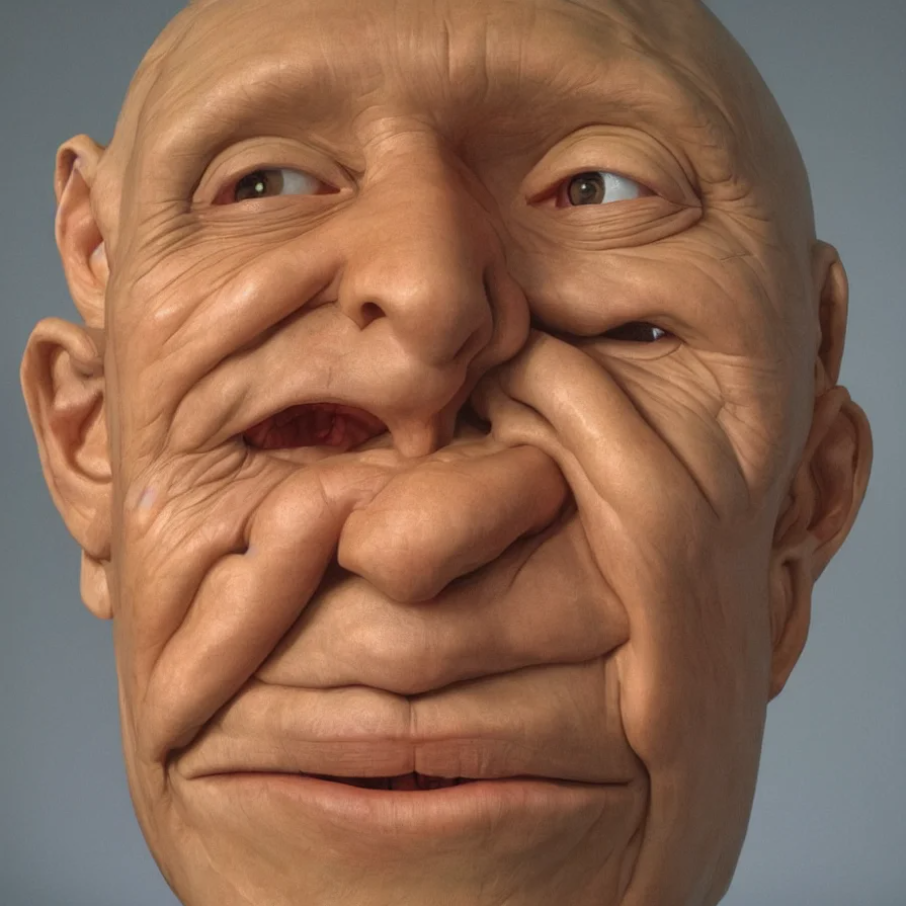
\includegraphics[scale=0.15]{face_deformada.png}
\caption{Imagem gerada por um prompt pedindo uma escultura hiperrealista de uma face humana. Encontrada no \href{https://lexica.art/prompt/10023e09-97d2-4ba3-8e01-4ee149a42c6f}{Lexica}.}
\end{figure}


A empresa OpenAI possui o gerador de imagens \textit{DALL-E}, que possui uma quantidade finita de geração de imagens gratuitas por mês. Após esta quantidade se esgotar é necessário pagar por prompts para gerar novas imagens, criando uma pequena barreira para aqueles que querem gerar imagens. O Google possui um gerador de imagens chamado \textit{Imagen}, mas este não está aberto ao público.



Além desses geradores ganhou notoriedade o método Stable Diffusion, difundido pela empresa Stability AI. A empresa, chefiada pelo CEO Emad Mostaque, foca no desenvolvimento open source de Stable Diffusion. Mostaque diz que a iniciativa open source é sobre "colocar o controle nas mãos das pessoas que construirão e estenderão a tecnologia." Entretanto, isso significa colocar \textbf{todas} essas capacidades nas mãos do público, para o bem ou para o mal.



Um dos problemas do Stable Diffusion é que não existem restrições sobre o tipo de conteúdo que pode ser gerador. Outros geradores, como DALL-E e Imagen, possuem restrições severas nas palavras-chave e conteúdo que podem gerar, enquanto que o Stable Diffusion pode ser utilizado localmente. Uma vez na máquina local de um usuário, não existe como restringir o que é gerado. Isto torna muito mais fácil de gerar conteúdo violento e sexual, incluindo imagens de pessoas reais. Com Stable Diffusion, o caso mais comum até o momento são usuários gerando pornografia.



Essa situação é território essencialmente desconhecido, e não é claro quais serão as consequências de soltar um modelo como esse para o público. É fácil de imaginar os fins maliciosos para os quais essa tecnologia pode ser utilizada, mas isso não significa que essas previsões acontecerão.



Outro problema é o uso de imagens com direitos autorais utilizadas como treinamento e base para as imagens geradas pelo Stable Diffusion. Apesar da empresa Stability AI fazer alguns filtros, ela não filtra o uso de bancos de dados de direitos autorais. Como resultado, muitos vêem a habilidade de Stable Diffusion imitar o style e estética de artistas vivos. Não apenas uma brecha de direito autoral mas também ética.



O aspecto de direitos autorais adiciona uma nova dimensão às reclamações que ferramentas como Stable Diffusion estão tirando trabalhos de artistas humanos. Não apenas está roubando trabalhos de artistas como está fazendo isso através de contrabandear, por assim dizer, as habilidades que esses indivíduos necessitaram de horas e horas para aperfeiçoar.
